%%%%%%%%%%%%%%%%%%%%%%%%%%%%%%%%%%%%%%%%%%%%%%%%%%%%%%%%%%%%%%%%%%%%%%%%%%%%%%%%
%2345678901234567890123456789012345678901234567890123456789012345678901234567890
%        1         2         3         4         5         6         7         8

\documentclass[letterpaper, 10 pt, conference]{ieeeconf}  % Comment this line out if you need a4paper

%\documentclass[a4paper, 10pt, conference]{ieeeconf}      % Use this line for a4 paper

\IEEEoverridecommandlockouts                              % This command is only needed if 
                                                          % you want to use the \thanks command

\overrideIEEEmargins                                      % Needed to meet printer requirements.

% See the \addtolength command later in the file to balance the column lengths
% on the last page of the document

% The following packages can be found on http:\\www.ctan.org
\usepackage{graphics} % for pdf, bitmapped graphics files
\usepackage{epsfig} % for postscript graphics files
%\usepackage{mathptmx} % assumes new font selection scheme installed
%\usepackage{times} % assumes new font selection scheme installed
\usepackage{amsmath} % assumes amsmath package installed
\usepackage{amssymb}  % assumes amsmath package installed
\usepackage{graphicx}

\usepackage{xcolor}

\bibliographystyle{IEEEtran}
\graphicspath{ {images/} }
\newtheorem{theorem}{Theorem}
\newtheorem{corollary}{Corollary}
\newtheorem{lemma}{Lemma}
\newtheorem{remark}{Remark}

\title{\LARGE \bf
A Risk-Sensitive Finite-Time Reachability Problem for Safety of Stochastic Dynamic Systems}

\author{Margaret P. Chapman$^{1}$, Jonathan P. Lacotte$^{2}$, Donggun Lee$^{3}$, Kevin Smith$^{4}$, Victoria Cheng$^{5}$,\\ 
Jaime Fernandez-Fisac$^{1}$, Aviv Tamar$^{1}$, Susmit Jha$^{6}$, Claire J. Tomlin$^{1}$% <-this % stops a space
\thanks{$^{1}$M.C., J.F., A.T., and C.T. are with the Department of Electrical Engineering and Computer Sciences, University of California, Berkeley, USA.
        {\tt\small chapmanm@berkeley.edu}}%
\thanks{$^{2}$J.L. is with the Department of Aeronautics and Astronautics, Stanford University, USA.
        }%
\thanks{$^{3}$D.L. is with the Department of Mechanical Engineering, University of California, Berkeley, USA.
        }%
\thanks{$^{4}$K.S. is with OptiRTC, Inc. and the Department of Civil and Environmental Engineering, Tufts University, USA.
        }%
\thanks{$^{5}$V.C. is with the Department of Civil and Environmental Engineering, University of California, Berkeley, USA.
        }%
\thanks{$^{6}$S.J. is with SRI International, Menlo Park, California, USA.
		}%
}

\begin{document}

\maketitle
\thispagestyle{empty}
\pagestyle{empty}

%%%%%%%%%%%%%%%%%%%%%%%%%%%%%%%%%%%%%%%%%%%%%%%%%%%%%%%%%%%%%%%%%%%%%%%%%%%%%%%%
\begin{abstract}
A classic reachability analysis problem for safety of dynamic systems is to compute the set of initial states from which 
the state trajectory is guaranteed to stay inside a given constraint set over some time horizon. 
In this paper, we leverage existing theory in reachability analysis and risk measures 
to formulate a \textit{risk-sensitive} reachability problem for safety of stochastic dynamic systems under non-adversarial disturbances
over a finite time horizon.
We provide two key contributions to reachability literature. 
First, our formulation accounts for rare high-consequence events by posing the optimal control problem in terms of a risk measure, 
called \textit{Conditional Value-at-Risk} (CVaR).
Stochastic reachability does not explicitly account for rare high-consequence events,
since the optimal control problem is posed in terms of the expectation operator.
Second, our formulation quantifies the distance between the boundary of the constraint set and the state trajectory in a stochastic setting. 
Stochastic reachability quantifies the probability that the state trajectory stays within the constraint set,
and Hamilton-Jacobi reachability quantifies the distance between the boundary of the constraint set and the state trajectory
in a deterministic setting.
We define a \textit{risk-sensitive safe set} as the set of initial states from which the risk of extreme constraint violation
can be made small via an appropriate control policy, where risk is quantified using CVaR.
We show that certain risk-sensitive safe sets enjoy probabilistic safety guarantees.
We provide a dynamic programming algorithm to compute under-approximations for risk-sensitive safe sets
and prove the correctness of the algorithm under the assumption of finite probability spaces. 
Our proof is a key contribution to reinforcement learning literature, as it does not require the assumption of strong duality,
which was required in a previous paper.
Finally, we demonstrate the utility of risk-sensitive reachability analysis as a design tool for stormwater infrastructure,
which is required to operate safely in the presence of rainfall uncertainty.
\end{abstract}
% Premise (hypothesis): A description of the problem being addressed, and the basic idea to address it. For an applications article, this would be a description of what the application was designed to do.
% Process (experiments): A description of what the authors actually did. For an application article, this would be the detail of the application itself; for a design article, the thought process that went in to the design.
% Outcome (results): What the experiment produced, or how the application performed, or the final design (for a design article).
% Conclusion: A summary of the lessons learned from the paper.
%%%%%%%%%%%%%%%%%%%%%%%%%%%%%%%%%%%%%%%%%%%%%%%%%%%%%%%%%%%%%%%%%%%%%%%%%%%%%%%%
\section{Introduction}
Reachability analysis is a formal verification method based on optimal control theory that can be used to prove 
safety or performance properties of dynamic systems~\cite{bansal2017hamilton}.
A classic reachability problem for safety is to compute the set of initial states from which 
the state trajectory is guaranteed to stay inside a given constraint set over some time horizon.
 
 
 
Typically, the dynamic system has a control signal to be designed to ensure constraint satisfaction 
and an uncertain disturbance signal that may try to prevent constraint satisfaction (i.e., is \textit{adversarial}). 
The guarantees enjoyed by the states of the safe set are either deterministic or probabilistic in nature, 
depending on what we assume about the system dynamics.

For example, we may assume that the control and disturbance signals are bounded, 
and we may not specify their probability distributions; in this case,
the dynamics are said to be \textit{nondeterministic}~\cite{mitchell2005toolbox}.
If the dynamics are nondeterministic and the disturbance signal is adversarial, then the safe set may be defined as the set of states from which the system can 
start, such that for any disturbance signal,
there exists a control signal that ensures constraint satisfaction (see~\cite{EECS-2018-41}, Sec. 2.2.1).
The safety guarantee is deterministic in this case, which has been studied extensively and applied mainly to vehicles (see~\cite{bansal2017hamilton} and the references therein). 

In contrast, we may assume that the state of the system is a random variable that evolves according to some probability distribution 
(e.g., see~\cite{bertsekas2005dynamic}, Sec. 1.2); here the dynamics are said to be \textit{stochastic}.
If the dynamics are stochastic and the disturbance input is adversarial, 
then the safe set may be defined as the set of states from which the system can start, such that for any disturbance signal,
there exists a control signal that ensures constraint satisfaction with sufficiently high probability (e.g., see~\cite{kamgarpour2011discrete}).
If the dynamics are stochastic and the disturbance input is non-adversarial (i.e., behaves as random noise),
then the safe set may be defined as the set of states from which the system can start, such that there exists a control signal 
that ensures constraint satisfaction with sufficiently high probability (e.g., see~\cite{summers2010verification} and~\cite{abate2008probabilistic}).
In these last two examples, the safety guarantees are probabilistic.

Whether the safety guarantee is deterministic or probabilistic in nature, 
its essential purpose is to inform decision-making in an uncertain world.
The key distinction between deterministic and probabilistic safety guarantees is how the uncertainty is quantified, and 
whether we assume a pessimistic world, where the uncertainty is adversarial, 
or a realistic world, where the uncertainty behaves as random noise.
In this paper, we develop a framework for reachability theory that lies on the spectrum between pessimism and realism,
by leveraging the theory of risk from finance and mathematics. 

Risk may be defined qualitatively as ``danger, or the possibility of danger, defeat, or loss"~\cite{riskdef}.
To quantify risk, the mathematical concept of a \textit{risk measure} has been developed.
A risk measure is a function that maps a random variable, $X$, representing loss into the real line,
according to the risk associated with $X$ (see~\cite{shapiro2009lectures}, Sec. 6.3; see~\cite{kisiala2015conditional}, Sec. 2.2).
Risk-sensitive optimization algorithms, which minimize the risk of predicted losses via a risk measure,
have been receiving more attention in the communities of applied mathematics~\cite{ruszczynski2010risk}, reinforcement learning~\cite{osogami2012robustness},~\cite{chow2015risk},~\cite{ratliff2017risk}, and optimal control~\cite{chow2014framework}.
Optimization programs that appreciate risk are desirable due to the limitations of alternative methods.
In particular, formulations that minimize worst-case losses under adversarial disturbances
may produce conservative results with limited practical utility, and formulations that minimize expected losses under random disturbances do not account for low-probability extreme events~\cite{chow2014framework},~\cite{jha2018safe}. 
On the other hand, risk-sensitive formulations have the potential to generate decisions that can be used in practice and that also protect
against particularly damaging outcomes~\cite{serraino2013conditional}.

In this paper, we leverage existing computational results for a particular risk measure, called \textit{Conditional Value-at-Risk} (CVaR),
to propose a framework for risk-sensitive reachability analysis. 
CVaR is a well-justified choice for several reasons.
CVaR is a \textit{coherent risk measure}, meaning that it satisfies several intuitive axioms, such as \textit{subadditivity},
which can be interpreted as ``diversification decreases risk" (see~\cite{kisiala2015conditional}, Sec. 2.2).
On finite probability spaces, coherent risk measures are expectations that have been maximized over a collection of perturbed probability distributions,
or expectations that have been made more robust to large losses~\cite{chow2014framework},~\cite{shapiro2009lectures},~\cite{chow2015risk},~\cite{artzner1999coherent}.
Recent work~\cite{chow2015risk} provides an algorithm to minimize the Conditional Value-at-Risk of total cost over time, 
which we leverage to compute risk-sensitive safe sets. Further, probabilistic safety guarantees and 
risk-sensitive safety guarantees are closely related, if the risk measure is CVaR, as we shall explain in Sec.~\ref{lemmaconnection}.

We propose a formulation for risk-sensitive reachability with several desirable attributes. 
At a fixed confidence level for CVaR, our formulation partitions the state space into regions of
varying degrees of safety quantified via the extent of constraint violation likely to be attained by the stochastic dynamic system.
Quantification of varying degrees of safety is a feature of safety guarantees for non-deterministic systems (see~\cite{EECS-2018-41}, Eq. 2.3) 
but not for stochastic systems currently. Existing safety guarantees for stochastic systems are binary, meaning that they encode whether the system is likely to be inside or outside a given set
(e.g., see~\cite{abate2008probabilistic},~\cite{summers2010verification}, and~\cite{kamgarpour2011discrete}).
Our formulation, however, provides a non-binary quantification of safety for stochastic systems,
which is particularly useful when constraint violation is not catastrophic (e.g., routine flooding of a pond after a large storm).
Further, our formulation inherits the benefits of risk-sensitive optimization and the benefits of reachability theory. 
By using a risk measure, our formulation may protect against rare harmful outcomes,
which are ignored by reachability formulations that provide safety guarantees in expectation (e.g.,~\cite{abate2008probabilistic},~\cite{summers2010verification}, and~\cite{kamgarpour2011discrete}),
and may also avoid unnecessary conservatism, which is a common limitation of deterministic safety guarantees (e.g., see~\cite{bansal2017hamilton}).
Like existing reachability methods, our formulation provides a comprehensive characterization of the state space in terms of safety.
This is not provided by recent work in risk-sensitive optimization, which computes optimal paths emanating from different initial conditions separately (e.g., see~\cite{chow2014framework} and~\cite{chow2015risk}).
A comprehensive safety characterization of the state space may be used 
to inform the cost-effective design of infrastructure that must withstand rare extreme storms,
to reduce overly conservative error bounds that arise in safe dynamic motion planning (e.g.,~\cite{herbert2017fastrack}), 
and to increase the amount of time that an autonomous vehicle can operate safely while simultaneously optimizing for performance.

Our formulation also inherits the disadvantages of risk-sensitive optimization and reachability analysis.
Since we evoke existing methods for risk-sensitive optimization, we are required to assume finite probability spaces.
Since we are not yet learning probability mass functions on-line, we assume that estimates of these functions are available, which is the case for evaluating designs of stormwater infrastructure
but not the case for real-time motion planning of a vehicle. Further, like existing methods for risk-sensitive optimization and reachability, 
our formulation generally requires a dynamic programming algorithm that is computationally expensive.

%every state contained in the risk-sensitive safe set that we will define enjoys a probabilistic safety guarantee, to be discussed in Sec.~\ref{lemmaconnection}. 
%We are interested in developing a framework for risk-sensitive reachability theory to inform decision-making in an uncertain world, where it may not be sensible to ensure safety by assuming worst-case circumstances.
% Want to quantify varying degrees of safety in a way that realistically (rather than pessimistically) appreciates/prepares for low-probability extreme events through the use of a financial risk measure (i.e., a ``robustified" expected value).
% Extends upon HJ Reachability analysis~\cite{mitchell2005time}, \cite{bansal2017hamilton} because it allows for stochastic dynamic systems.
% Extends upon Stochastic Reachability analysis~\cite{summers2010verification}, \cite{kamgarpour2011discrete} because it quantifies varying degrees of safety.

\section{System Model}\label{model}
The system model is a special case of the model given by~\cite{bertsekas2005dynamic} in Sec. 1.2.
We consider a stochastic discrete-time dynamic system over a finite time horizon,
\begin{equation}
x_{k+1} = f_k(x_k,u_k,w_k), \text{ }\text{ } k = 0, 1, \dots, T-1,
\label{sys}\end{equation}
such that $x_k \in S$ is the state of the system at time $k$,
$u_k \in C$ is the control input at time $k$, and
$w_k \in D_k = \{d_1^k,\dots,d_N^k\}$ is the random disturbance input at time $k$ defined over a finite probability space.
The control input is not random, but the state generally is random because it depends on random disturbances.
The initial condition, $x_0$, is not random for simplicity.
The collection of admissible control policies is,
\begin{equation}
\Pi = \{ (\mu_0, \mu_1, \dots, \mu_{T-1}), \text{ such that } \mu_k: S\rightarrow C \}.
\end{equation}
The random disturbance at time $k$, $w_k$, is characterized by a 
time-dependent probability mass function that is independent of any control policy, $\pi \in \Pi$, and other disturbances, $w_{\not k} = (w_0, \dots, w_{k-1}, w_{k+1}, \dots, w_{T-1})$.\footnotemark
\footnotetext{The probability mass function may be state-dependent as well.}
Formally, we have
\begin{equation}\begin{aligned}
P_k( w_k = d^k_j | x_k ) & = p_j^k, \\
\textstyle\sum_{j=1}^N p_j^k & = 1, \text{ } p_j^k \geq 0, \\
P_k( w_k = d^k_j | x_k, \pi, w_{\not k}) & = P_k( w_k = d^k_j | x_k ),
\end{aligned}\end{equation}
for each disturbance sample $j = 1,\dots,N$ and each time point $k = 0, 1, \dots, T-1$.
We are given a (non-empty) constraint set, $\mathcal{K} \subset S$, and the safety criterion that 
the state of the system should stay inside $\mathcal{K}$ over time.
For example, if our application is the flow of water through a network of ponds and streams, $\mathcal{K}$ may indicate that the water does not overflow the banks during a storm event.

\section{Problem Statement}
The goal of this paper is to design an algorithm that computes a \textit{risk-sensitive safe set} 
for a system of the form specified in Sec.~\ref{model}.
A risk-sensitive safe set is, informally, the set of initial conditions of the system, from which there is small risk of large constraint violations over time.

We quantify risk using the well-established risk measure, \textit{Conditional Value-at-Risk} (CVaR), which is equal to,
\begin{equation}
\text{CVaR}_\delta(Z) = {\underset{c \in \mathbb{R}}\min} \text{ }\Big\{ c + \frac{1}{\delta}\mathbb{E}\big[\max\{Z-c,0\}\big] \Big\},
\label{cvareqn}
\end{equation}
where $\delta \in (0,1)$, and $Z$ is a random variable representing loss~\cite{rockafellar2000optimization}.\footnotemark
\footnotetext{Definitions of CVaR are presented in various forms. The original paper is~\cite{rockafellar2000optimization}.
Other references on CVaR include~\cite{serraino2013conditional} (see Eq. (9)) and~\cite{kisiala2015conditional}.}
If $Z$ is a continuous random variable, then $\text{CVaR}_\delta(Z)$ is the expected value of $Z$ over large realizations of $Z$,
where the meaning of large is based on $\delta$ (Fig.~\ref{cvar}).

\begin{figure}[thpb]
      \centering
      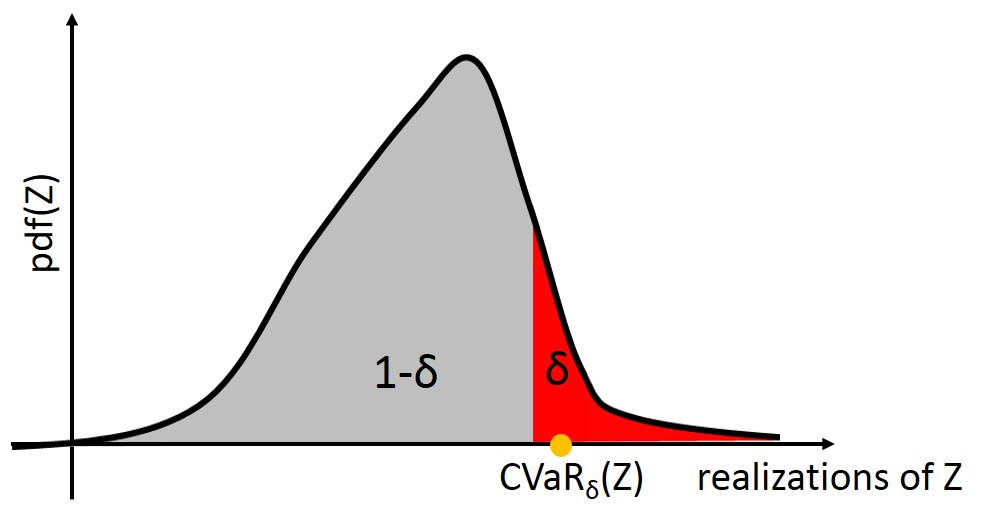
\includegraphics[scale=0.5]{cvar.jpg}
      \caption{An illustration of $\text{CVaR}_\delta(Z) \in \mathbb{R}$, if $Z$ is a continuous random variable. 
	  The graph shows the probability density function of $Z$ versus the realizations of $Z$.
	  The area of the right portion under the curve, shown in red, is $\delta \in (0,1)$.	  
	  The area of the left portion under the curve, shown in grey, is $1-\delta$.
	  $\text{CVaR}_\delta(Z)$ is the expectation of the values along the right portion under the curve, indicated by a yellow circle.}
      \label{cvar}
\end{figure}

We quantify the extent of constraint violation via a surface function that characterizes the constraint set, $\mathcal{K}$.
Let $g: S \rightarrow \mathbb{R}$ satisfy,
\begin{equation}
x \in \mathcal{K} \iff g(x) < 0,
\label{g}
\end{equation}
where we adopt the convention provided by~\cite{EECS-2018-41} in Eq. (2.3). 
The particular form of $g$ is chosen based on how safety of the system changes with distance to the boundary of $\mathcal{K}$ for the application at hand.
For example, if the relationship between safety and distance to the boundary of $\mathcal{K}$ is linear, 
then the signed distance function for $\mathcal{K}$ is a suitable choice for $g$ (Fig.~\ref{exg}, dotted).
However, if the relationship between safety and distance to the boundary of $\mathcal{K}$ is non-linear,
then a quadratic function may be more appropriate (Fig.~\ref{exg}, solid).

\begin{figure}[thpb]
      \centering
      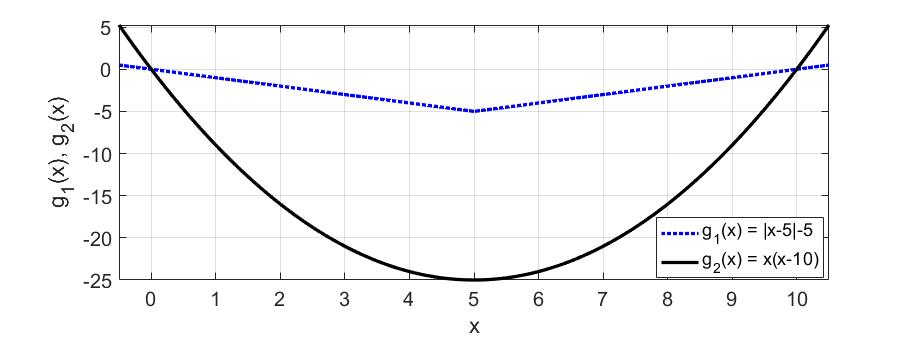
\includegraphics[scale=0.25]{examples_of_g.jpg}
      \caption{Different choices for the particular form of $g$, see~\eqref{g}, for an example constraint set, $\mathcal{K} = (0, 10)$. The relationship between
		safety and distance to the boundary of $\mathcal{K}$ is linear for $g_1(x) = |x-5|-5$ (dotted), and non-linear for $g_2(x) = x(x-10)$ (solid).
		For example, the degree of safety at $x=6$ characterized by the linear relationship is, $g_1(6) = -4$, since the closest distance 
		from $x=6$ to the boundary of $\mathcal{K}$ is 4, and $x=6$ is inside $\mathcal{K}$.}
      \label{exg}
\end{figure}

We are now ready to define the risk-sensitive safe set formally.
Let $\xi_y^\pi(k) \in S$ be the random state of the system at time $k$ that satisfies~\eqref{sys} under a given control policy $\pi \in \Pi$,
starting from a given (non-random) state $y \in S$ at time 0.  
The maximum extent of constraint violation attained by the system under policy $\pi \in \Pi$, starting from initial condition $y \in S$, 
is given by the random variable,
\begin{equation}
X_y^\pi = {\underset{k \in \{0, \dots, T\}}\max} \Big\{ g\big(\xi_y^\pi(k)\big) \Big\},
\label{xpiy}\end{equation}
where $g$ satisfies~\eqref{g}.
For any $\delta \in (0,1)$, the risk-sensitive safe set is,
\begin{equation} \begin{aligned}
\mathcal{U}_\delta := &  \Big\{y \in S\text{ }|\text{ }\exists \pi \in \Pi \text{ such that } \text{CVaR}_\delta\left(X_y^\pi\right) < 0 \Big\} \\
= & \Big\{y \in S \text{ }|\text{ } {\underset{\pi \in \Pi}\min}\text{ } \big\{\text{CVaR}_\delta\left(X_y^\pi\right)\big\} < 0 \Big\},
\label{U}\end{aligned}\end{equation}
where the random variable, $X_y^\pi$, is defined in~\eqref{xpiy},
and the conditional value-at-risk is taken with respect to the probability distribution of $(w_0, \dots, w_{T-1})$. 
To summarize, the risk-sensitive safe set is the set of initial conditions from which
the risk of large constraint violations can be made small by an appropriate control policy.
The problem addressed in this paper is how to compute~\eqref{U}.

\section{Properties of $\mathcal{U}_\delta$}
Here we present two key properties of the risk-sensitive safe set.
The first property is that every state in $\mathcal{U}_\delta$ enjoys a probabilistic safety guarantee.
To prove this property, we need the following result adopted from~\cite{shapiro2009lectures}.\\
\textcolor{blue}{SJ: The simplified proof is using $\delta = 1 - \alpha$. I suggest we use this notation throughout the paper. }\\
\begin{lemma}\label{lemma1}
 Let $\delta \in (0,1)$, and $Z$ be a random variable. If $\text{CVaR}_\delta(Z) < 0$, then $\mathbb{P}[Z\geq 0] < \delta$ (see~\cite{shapiro2009lectures}, Sec. 6.2.4).\footnotemark
\end{lemma}
\textcolor{blue}{\begin{proof} SJ: simplifying the proof below. 
\begin{align}
& \text{CVaR}_{1-\alpha}(Z) < 0 \nonumber \\ 
\iff & \frac{1}{1-\alpha} \mathbb{E}\big[\max\{Z-c,0\}\big] < -c \nonumber \\
\iff & \exists c \in \mathbb{R} \;\; c + \frac{1}{1-\alpha}\mathbb{E}\big[\max\{Z-c,0\}\big] < 0 \; [\text{using }~\eqref{cvareqn}] \nonumber \\
\iff & \mathbb{E}\big[\max\{Z-c,0\}\big] < -c(1-\alpha) \label{proofeqn1}
\end{align} 
Now, the LHS of the inequality,  $\mathbb{E}\big[\max\{Z-c,0\}\big] \geq 0$ because the expectation of non-negative values cannot be negative. Consequently, the RHS of the inequality must also be non-negative, that is, $-c(1-\alpha) \geq 0$, that is, $c \leq 0$ since $1-\alpha \geq 0$. So, we can rewrite  inequality~\eqref{proofeqn1} using $ a = -c \geq 0$ as follows: 
\begin{align}
& \mathbb{E}\big[\max\{Z+a,0\}\big] < a(1-\alpha), \; \text{where} \; a \geq 0 \nonumber \\
\iff & \; \frac{1}{a}\mathbb{E}\big[\max\{Z+a,0\}\big] < 1-\alpha, \; \text{where}  \; a \geq 0 \label{proofeqn2}
\end{align}
Using Markov's Inequality,
$\mathbb{P}\big[\max\{Z+a,0\} \geq a \big] \leq  \frac{1}{a}\mathbb{E}\big[\max\{Z+a,0\}\big]$. Combining with inequality~\eqref{proofeqn2},\\
\begin{align}
& \mathbb{P}\big[\max\{Z+a,0\} \geq a \big] \leq  \frac{1}{a}\mathbb{E}\big[\max\{Z+a,0\}\big] < 1-\alpha \nonumber \\
\Rightarrow \;\; & \mathbb{P}\big[\max\{Z+a,0\} \geq a \big] < 1-\alpha \label{proofeqn3}
\end{align}
Now, $Z \geq 0 \iff Z+a \geq a \iff \max\{Z+a,0\} \geq a $ since $a \geq 0$, and so,\\
$\mathbb{P}\big[Z \geq 0\big] = \mathbb{P}\big[\max\{Z+a,0\} \geq a\big]$.
Combining with the inequality~\eqref{proofeqn3},
\begin{align*}
& \mathbb{P}\big[Z \geq 0\big] = \mathbb{P}\big[\max\{Z+a,0\} \geq a\big] < 1-\alpha \\
\iff \;\; & \mathbb{P}\big[Z \geq 0\big] < 1-\alpha 
\end{align*}
\end{proof}
The only one-sided implication is in the use of Markov's Inequality to get inequality~\eqref{proofeqn2}, and this corresponds to the approximation gap in using 
 $\text{CVaR}_{1-\alpha}(Z) < 0$
 to approximate $\mathbb{P}[Z\geq 0] < 1-\alpha$.\\}
%% sj: end new proof
\footnotetext{Ref.~\cite{shapiro2009lectures} indicates that the constraint, $\text{CVaR}_\delta(Z) \leq 0$, gives a conservative approximation of the chance constraint, $\mathbb{P}[Z > 0] \leq \delta$. %pp. 257-258 
$\text{CVaR}_\delta(Z) \leq 0$ is written as ``$\text{AV@R}_\alpha(Z_x) \leq 0$'' in~\cite{shapiro2009lectures}, see (6.24).
$\mathbb{P}[ Z > 0] \leq \delta$ is equivalent to $\mathbb{P}[ Z\leq 0] \geq 1 - \delta$, 
which is written as ``$\text{Pr}(Z_x \leq 0) \geq 1 - \alpha$" in~\cite{shapiro2009lectures}, see text below (6.18).}
The next corollary indicates that every state in $\mathcal{U}_\delta$ enjoys a probabilistic safety guarantee.
\begin{corollary}
$\mathcal{U}_\delta$, as defined in~\eqref{U}, is a subset of $\mathcal{S}_\delta$,
\begin{equation}
\mathcal{S}_\delta := \Big\{y \in S\text{ }|\text{ }\exists \pi \in \Pi\text{, } \mathbb{P}\left[\forall k \in \mathbb{T}\text{, }\xi_y^\pi(k) \in \mathcal{K} \right]  > 1-\delta \Big\}, \\
\label{S}\end{equation}
where $\mathbb{P}$ is the probability measure for the state trajectory, and $\mathbb{T} = \{0, 1, \dots, T\}$ is the time horizon.
\end{corollary}
\begin{proof}
\textcolor{blue}{may want to remove this proof b/c it's not very important?}
Take $y \in \mathcal{U}_\delta$. Then, there exists $\pi \in \Pi$ such that $\text{CVaR}_\delta(X_y^\pi) < 0$, 
which implies $\mathbb{P}[X_y^\pi \geq 0] < \delta$ by Lemma~\ref{lemma1}.
After some algrebra using~\eqref{g} and~\eqref{xpiy},
\begin{equation}
\mathbb{P}[X_y^\pi \geq 0] = 1 - \mathbb{P}\left[\forall k \in \mathbb{T}\text{, } \xi_y^\pi(k) \in \mathcal{K} \right].
\end{equation}
So, $\exists \pi \in \Pi$ such that $\mathbb{P}\left[\forall k \in \mathbb{T}\text{, } \xi_y^\pi(k) \in \mathcal{K} \right] > 1- \delta$, implying that $y \in \mathcal{S}_\delta$.
\end{proof}
The second key property of the risk-sensitive safe set, $\mathcal{U}_\delta$, is, as $\delta$ decreases,
the states of $\mathcal{U}_\delta$ enjoy a stronger probabilistic safety guarantee, and $\mathcal{U}_\delta$ becomes smaller.
\begin{lemma}\label{lemma2}
Let $1>\delta_1 \geq \delta_2>0$. Then, $\mathcal{S}_{\delta_2} \supset \mathcal{S}_{\delta_1}$,
and $\mathcal{U}_{\delta_2} \supset \mathcal{U}_{\delta_1}$, where $\mathcal{U}_{\delta}$ is given by~\eqref{U}
and $\mathcal{S}_{\delta}$ is given by~\eqref{S}. 
\end{lemma}
\begin{remark}{Remark}

\end{remark}




Please see Table~\ref{terms} for a summary of relevant notation.

\textit{Problem 1}. An important problem is to compute the set of initial states for which there exists an admissible control policy that keeps
the system inside the constraint set over time with sufficiently high probability. The \textit{safe set} with confidence $1-\delta \in (0,1)$ is defined as,
\begin{equation}
\mathcal{S}(\delta) := \{ x \in S\text{ }|\text{ } \exists \pi \in \Pi \text{ such that } \mathbb{P}[ \forall k \in \mathbb{T}\text{, } \xi_x^\pi(k)\in \mathcal{K}] > 1-\delta \}.
\end{equation}

\begin{table}
\begin{center}
\caption{}
\begin{tabular}{| p{1.5cm} | p{6cm} | p{7cm} |}
\hline
Symbol & Definition & Expression (if applicable) \\ \hline
$g$ & Surface function that characterizes the constraint set, $\mathcal{K}$ & $x \in \mathcal{K} \iff g(x) < 0$ \\ \hline
$C$ & Set of possible values for the control input & \\ \hline
$D_k$ & Sample space for the random disturbance input at time $k$ & $D_k := \{d_1^k, d_2^k, \dots, d_N^k\}$ \\ \hline
$S$ & Set of (continuous) states  & $S := \mathbb{R}^n$ \\ \hline
$\mathcal{K}$ & Constraint set & $\mathcal{K} \subset S$ \\ \hline
$\Pi$ & Set of admissible control policies & $\Pi := \{ (\mu_0, \mu_1, \dots, \mu_{T-1}), \text{ such that } \mu_k: S\rightarrow C \}$ \\ \hline
$\mathbb{P}$ & The probability measure with respect to $(w_0, w_1, \dots, w_{T-1})$ & \\ \hline
$\mathbb{T}$ & Finite discrete time horizon & $\mathbb{T} := \{0, 1, \dots, T\}$ \\ \hline
$\xi_x^\pi(k)$ & Random state at time $k$ under (fixed) policy $\pi$, starting from (fixed) initial condition, $x \in S$, at time 0 &  \\ \hline
\end{tabular}
\begin{flushleft}\end{flushleft}
\label{terms}
\end{center}
\end{table}

\section{Relation between Probablistic Safety and CVaR safety}\label{lemmaconnection}







\section{Conclusion}\label{conclusion}

\section*{ACKNOWLEDGMENT}
We thank Mo Chen and Jaime Fisac for discussions.
M.C. is supported in part by a NSF Graduate Research Fellowship.
This work is supported in part by NSF CPS 1740079.

%\section*{APPENDIX}\label{appendix}

\addtolength{\textheight}{-2cm}   % This command serves to balance the column lengths
                                  % on the last page of the document manually. It shortens
                                  % the textheight of the last page by a suitable amount.
                                  % This command does not take effect until the next page
                                  % so it should come on the page before the last. Make
                                  % sure that you do not shorten the textheight too much.

\bibliography{references}

\end{document}
